\section{Bilayer graphene}

In the tight-binding description of bilayer graphene, we take into account $2p_z$ orbitals on the four atomic sites in the unit cell, labelled as $j = A_1, B_1, A_2, B_2$. Then, the transfer integral matrix of bilayer graphene is a $4\times 4$  matrix given by \cite{McCann_2013}

\begin{equation}
    H(\vect k)=
    \begin{bmatrix}
        E_{A_1} & -\gamma_0 F(\vect k) & \gamma_4 F(\vect k) & -\gamma_3 F(\vect k)\\
        -\gamma_0 F(\vect k) & E_{B_1} & -\gamma_1 & \gamma_4 F(\vect k)\\
        \gamma_4 F(\vect k) & \gamma_1 & E_{A_2} & -\gamma_0 F(\vect k)\\
        -\gamma_3 F(\vect k)& \gamma_4 F(\vect k)& -\gamma_0 F(\vect k) & E_{B_2}
    \end{bmatrix}
\end{equation}
\begin{figure}[h]
    \makebox[\textwidth][c]{
        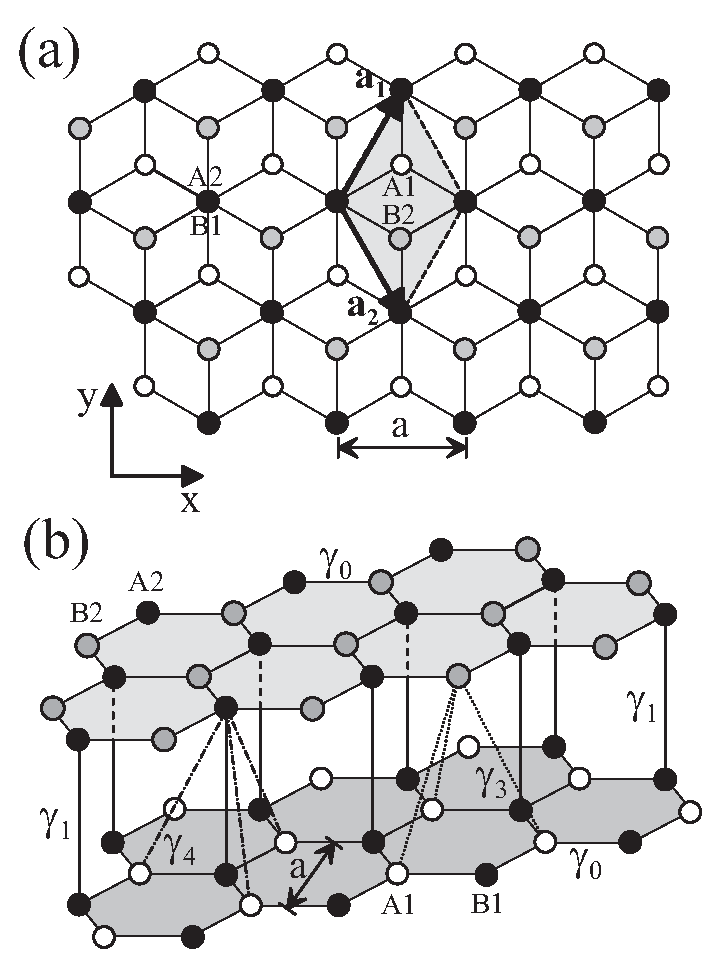
\includegraphics[width=.7\linewidth]{Immagini/graphene/bilayerlattice.eps}
        }%
    \caption{difference between the gapless and the gapped Dirac dispersion relation}
    \label{fig:bilayer-lattice}
\end{figure}
where the tight-binding parameters are defined as 
\begin{equation}
    \begin{split}
        \gamma_0=&-\braket{A_1|H}{B_1}=-\braket{A_2|H}{B_2} \\
        \gamma_1=&\braket{A_2|H}{B_1}  \\
        \gamma_3=&-\braket{A_1|H}{B_2}  \\
        \gamma_4=& \braket{A_1|H}{A_2}=\braket{B_1|H}{B_2} \\
    \end{split}
\end{equation}
The upper-right and lower-left square $2\times 2$ blocks of $H$ describe inter-layer coupling. Parameter $\gamma_1$ describes coupling between pairs of orbitals on sites that are directly above each other $B_1$ and $A_2$: since this is a vertical coupling, the corresponding terms in $H$ do not contain $F(\vect k)$ which describes in-plane hopping. The other $\gamma$ factors do have an in plane component, which causes the $F(\vect k)$ term to show up.\\
The overlap matrix $S$ form equation $\ref{eq:overlap}$ becomes in the bilayer case
\begin{equation}
    S=
    \begin{bmatrix}
        1 & s_0 F(\vect k) & 0&0\\
        s_0 F(\vect k)  &1&s_1&0\\
        0&s_1&1&s_0 F(\vect k)\\
        0&0&s_0 F(\vect k) &1
    \end{bmatrix}
\end{equation}
Here we only include two parameters: $s_0 = \braket{A_1}{B_1} = \braket{A_2}{B_2}$ describing non-orthogonality of intra-layer nearest-neighbours and $s_1= \braket{A_2}{B_1}$ describing non-orthogonality of orbitals on dimer sites A1 and B2. In principle, it is possible to introduce additional parameters analogous to $\gamma_3,\gamma_4$, etc., but generally they will be small and irrelevant, infact in the bilayer case it is common practice to neglect completely the overlap matrix if we are dealing with 